% !TeX root = construct.tex

\chapter{How to (Almost) Square a Circle}

\section{Approximations to $\pi$}

The Greeks first studied geometrical constructions that use a straightedge and compass. They were not able to solve three problems: trisecting an angle, duplicating a cube (given a cube, construct another cube with twice the volume) and squaring a circle (given a circle, construct a square with the same area). In the nineteenth century it was proved that these constructions are impossible.

It can be shown algebraically that given a line segment defined to have length $1$, the constructible numbers (lengths) are those obtainable from that line segment using the operators $+,-,\times,\div,\surd$. Since cube roots cannot be constructed, it follows that it is impossible to duplicate an arbitrary cube, because to duplicate a cube of volume $1$ requires solving the equation $x^3-2=0$, that is, constructing the length $\sqrt[3]{2}$. For the same reason, it is impossible to trisect an arbitrary angle, because to trisect $60^\circ$ requires solving the cubic equation $8x^3-6x-1=0$.

The case of squaring the circle is more difficult and was not solved until 1882. The area of the unit circle is $\pi r^2=\pi$, so it is required to construct a square whose side is $\sqrt{\pi}$. However, $\pi$ is \emph{transcendental}, meaning that it is not the solution of \emph{any} algebraic equation. The proof is extremely complex involving concepts from analysis and complex numbers.

There are simple approximations to $\pi$, in particular:
\[
\frac{355}{113}=3.14159292\,,
\]
which differs from $\pi\approx 3.14159265$ by only $2.67\times 10^{-7}$. Consider the radius of the earth at the equator which is $6,378.1$ km. Computing the circumference using $355/113$ gives $40,074.78761$ km, while using $\pi$ the result is $40,074.78421$ km, a difference of less than $4$ meters!

The rational number $355/113$ could be constructed by extending the line segment of length one $113$ times, extending it again to obtain a line segment of length $355$, and constructing a segment whose length is the quotient of  the two. This note presents a short construction of $355/113$ published by Ramanujan in the \emph{Journal of the Indian Mathematical Society}, 1913, p. 138. We present the construction in incremental stages, asking you to perform the computations in each stage as exercises. Answers are given at the end of the note, followed by Ramanujan's article.

Ramanujan (1887--1920) grew up in what is now the state of Tamil Nadu in India, but quickly advanced beyond the mathematical level of the local schools and colleges. He sent his work to the English mathematician G.H. Hardy who invited him to England. Ramanujan arrived in 1914 but could not return to India until after World War I. He suffered greatly from the cold climate and unfamiliar food and died at age $32$ shortly after returning to India. Ramanujan's mathematics is still the subject of research one hundred years later. A biography of Ramanujan is: Robert Kanigel. \emph{The Man Who Knew Infinity: A Life of the Genius Ramanujan}, 1991.

\newpage

%%%%%%%%%%%%%%%%%      First

\begin{center}
\textbf{\Large Stage 1}
\end{center}

\begin{itemize}
\item Construct a unit circle centered at $O$ and let $PR$ be a diameter.
\item Mark point $H$ that bisects $PO$ and mark point $T$ that trisects $RO$.
\item Construct a perpendicular at $T$. Its intersection with the circle is $Q$.
\item Construct a chord $RS=QT$.
\end{itemize}

\begin{center}
\begin{tikzpicture}[scale=.9]
% Draw circle and horizontal diameter
\draw[name path=circle] (0,0)  coordinate (o) node[below] {$O$} circle[radius=5cm];
\draw (-5,0) coordinate (p) node[left] {$P$} -- (5,0) coordinate (r) node[right] {$R$};
\fill (o) circle (1pt);
\fill (p) circle (1pt);
\fill (r) circle (1pt);
\fill (-2.5,0) coordinate (h) node[below] {$H$} circle (1pt);
\fill (10/3,0) coordinate (t) node[below] {$T$} circle (1pt);
\path (p) -- node[above,xshift=12pt] {$1/2$} (h) -- node[above] {$1/2$} (o) -- node[above] {$2/3$} (t) -- node[above] {$1/3$} (r);
% Draw perpendicular TQ
\path[name path=tq] (t) -- +(0,5);
\path[name intersections={of=tq and circle,by=q}];
\draw (t) -- node[left] {$a$} (q) node[above] {$Q$};
\fill (q) circle (1pt);
% Draw chord RS
\path[name path=rcirc] (r) let \p1 = ($ (t) - (q) $) in circle ({veclen(\x1,\y1)});
\path[name intersections={of=rcirc and circle,by=s}];
\draw (r) -- node[left] {$a$} (s);
\fill (s) node[above right] {$S$} circle (1pt);
\draw (p) -- node[above] {$b$} (s);
\end{tikzpicture}
\end{center}

\exer
Construct the length $TR=\displaystyle\frac{1}{3}$.


\exer{}
Compute the length of $QT$.


\exer{}
Compute the length of $PS$.


\exer{}
Construct chord $RS=QT$.


\newpage

%%%%%%%%%%%%%%%%%      Second

\begin{center}
\textbf{\Large Stage 2}
\end{center}

\begin{itemize}
\item Construct $NT$ and $OM$ parallel to $RS$.
\end{itemize}

\begin{center}
\begin{tikzpicture}[scale=.9]
% Draw circle and horizontal diameter
\draw[name path=circle] (0,0)  coordinate (o) node[below] {$O$} circle[radius=5cm];
\draw (-5,0) coordinate (p) node[left] {$P$} -- (5,0) coordinate (r) node[right] {$R$};
\fill (o) circle (1pt);
\fill (p) circle (1pt);
\fill (r) circle (1pt);
\fill (-2.5,0) coordinate (h) node[below] {$H$} circle (1pt);
\fill (10/3,0) coordinate (t) node[below] {$T$} circle (1pt);
% Draw chord RS and line PS
\path[name path=tq] (t) -- +(0,5);
\path[name intersections={of=tq and circle,by=q}];
\path[name path=rcirc] (r) let \p1 = ($ (t) - (q) $) in circle ({veclen(\x1,\y1)});
\path[name intersections={of=rcirc and circle,by=s}];
\draw (r) -- node[left] {$a$} (s);
\fill (s) node[above right] {$S$} circle (1pt);
\draw[name path=ps] (p) -- node[above right,xshift=8pt,yshift=8pt] {$b$} (s);
% Draw TN
\path[name path=tn] (t) -- +($(s)-(r)$);
\path[name intersections={of=ps and tn,by=n}];
\draw (t) -- (n);
\fill (n) node[above] {$N$} circle (1pt);
% Draw OM
\path[name path=om] (o) -- +($(s)-(r)$);
\path[name intersections={of=ps and om,by=m}];
\draw (o) -- (m);
\fill (m) node[above left] {$M$} circle (1pt);
% Label PM and MN
\path (p) -- node[below,xshift=12pt,yshift=4pt] {$c$} (m);
\path (m) -- node[below,xshift=8pt,yshift=4pt] {$d$} (n);
\end{tikzpicture}
\end{center}

\exer{}
Compute the length of $PM$.


\exer{}
Compute the length of $MN$.


\newpage

%%%%%%%%%%%%%%%%%      Third

\begin{center}
\textbf{\Large Stage 3}
\end{center}


\begin{itemize}
\item Construct the chord $PK=PM$.
\item Construct the tangent $PL=MN$.
\item Connect the points $K,L,R$.
\end{itemize}

\begin{center}
\begin{tikzpicture}[scale=.9]
% Draw circle and horizontal diameter
\draw[name path=circle] (0,0)  coordinate (o) node[below] {$O$} circle[radius=5cm];
\draw (-5,0) coordinate (p) node[left] {$P$} -- (5,0) coordinate (r) node[right] {$R$};
\fill (o) circle (1pt);
\fill (p) circle (1pt);
\fill (r) circle (1pt);
\fill (-2.5,0) coordinate (h) node[below] {$H$} circle (1pt);
\fill (10/3,0) coordinate (t) node[below] {$T$} circle (1pt);
% Draw chord RS and line PS
\path[name path=tq] (t) -- +(0,5);
\path[name intersections={of=tq and circle,by=q}];
\path[name path=rcirc] (r) let \p1 = ($ (t) - (q) $) in circle ({veclen(\x1,\y1)});
\path[name intersections={of=rcirc and circle,by=s}];
\draw (r) -- (s);
\fill (s) node[above right] {$S$} circle (1pt);
\draw[name path=ps] (p) -- (s);
% Draw TN
\path[name path=tn] (t) -- +($(s)-(r)$);
\path[name intersections={of=ps and tn,by=n}];
\draw (t) -- (n);
\fill (n) node[above] {$N$} circle (1pt);
% Draw OM
\path[name path=om] (o) -- +($(s)-(r)$);
\path[name intersections={of=ps and om,by=m}];
\draw (o) -- (m);
\fill (m) node[above left] {$M$} circle (1pt);
\path (p) -- node[below,xshift=12pt,yshift=4pt] {$c$} (m);
\path (m) -- node[below,xshift=8pt,yshift=4pt] {$d$} (n);
% Draw chord PK
\path[name path=pkcirc] (p) let \p1 = ($ (p) - (m) $) in circle ({veclen(\x1,\y1)});
\path[name intersections={of=pkcirc and circle,by={k1,k}}];
\draw (p) -- node[right,xshift=-2pt,yshift=10pt] {$c$} (k) node[below left] {$K$};
% Draw tangent PL
\draw let \p1 = ($ (m) - (n) $), \n1 = {veclen(\x1,\y1)} in (p) -- node[left] {$d$} (-5,-\n1) coordinate (l) node[left] {$L$};
% Connect L and K to R
\draw (r) -- node[above] {$f$} (l) -- (k) -- node[below right] {$e$} cycle;
\end{tikzpicture}
\end{center}

\exer{}
What do you know about $\triangle PKR$? Compute the length of $RK$.


\exer{}
What do you know about $\triangle LPR$? Compute the length of $RL$.


\newpage

%%%%%%%%%%%%%%%%%      Fourth

\begin{center}
\textbf{\Large Stage 4}
\end{center}

\begin{itemize}
\item Mark the point $C$ such that $RC=RH$.
\item Construct $CD$ parallel to $KL$.
\end{itemize}

\begin{center}
\begin{tikzpicture}[scale=.9]
% Draw circle and horizontal diameter
\draw[name path=circle] (0,0)  coordinate (o) node[below] {$O$} circle[radius=5cm];
\draw (-5,0) coordinate (p) node[left] {$P$} -- (5,0) coordinate (r) node[right] {$R$};
\fill (o) circle (1pt);
\fill (p) circle (1pt);
\fill (r) circle (1pt);
\fill (-2.5,0) coordinate (h) node[below] {$H$} circle (1pt);
% Get values of PM and MN but don't draw
\coordinate (t) at (10/3,0);
\path[name path=tq] (t) -- +(0,5);
\path[name intersections={of=tq and circle,by=q}];
\path[name path=rcirc] (r) let \p1 = ($ (t) - (q) $) in circle ({veclen(\x1,\y1)});
\path[name intersections={of=rcirc and circle,by=s}];
\path[name path=ps] (p) -- (s);
\path[name path=tn] (t) -- +($(s)-(r)$);
\path[name intersections={of=ps and tn,by=n}];
\path[name path=om] (o) -- +($(s)-(r)$);
\path[name intersections={of=ps and om,by=m}];
% Draw chord PK
\path[name path=pkcirc] (p) let \p1 = ($ (p) - (m) $) in circle ({veclen(\x1,\y1)});
\path[name intersections={of=pkcirc and circle,by={k1,k}}];
\draw (p) -- (k) node[below left] {$K$};
% Draw tangent PL
\draw let \p1 = ($ (m) - (n) $), \n1 = {veclen(\x1,\y1)} in (p) -- (-5,-\n1) coordinate (l) node[left] {$L$};
% Connect L and K to R
\draw (r) -- node[above] {$f$} (l) -- (k) -- node[below right] {$e$} cycle;
% Find point C on RK
\coordinate (c) at ($(r)!7.5cm!(k)$);
\path (r) -- node[above, near end] {$g$} (c);
\fill (c) node[below] {$C$} circle (1pt);
% Draw CD
\path[name path=cd] (c) -- +($(l)-(k)$);
\path[name path=lr] (l) -- (r);
\path[name intersections={of=cd and lr,by=d}];
\draw (c) -- (d);
\fill (d) node[above,xshift=2pt] {$D$} circle (1pt);
\path (r) -- node[below,near end] {$h$} (d);
\end{tikzpicture}
\end{center}


\exer{}
Compute the length of $RC$.


\exer{}
Compute the length of $RD$.



\exer{}
Construct a square whose side is of length $RD$.


\exer{}
Compute $RD^2$, the area of the square, both as a fraction and as a decimal number.


\newpage

%%%%%%%%%%%%%%%%%      Fifth

\begin{center}
\textbf{\Large Summary}
\end{center}

Here is the complete construction with all lengths labeled.

\bigskip

\begin{center}
\begin{tikzpicture}[scale=1.2,align=left]
% Draw circle and horizontal diameter
\draw[name path=circle] (0,0)  coordinate (o) node[below] {$O$} circle[radius=5cm];
\draw (-5,0) coordinate (p) node[left] {$P$} -- (5,0) coordinate (r) node[right] {$R$};
\fill (o) circle (1pt);
\fill (p) circle (1pt);
\fill (r) circle (1pt);
\fill (-2.5,0) coordinate (h) node[below] {$H$} circle (1pt);
\fill (10/3,0) coordinate (t) node[below] {$T$} circle (1pt);
\path (p) -- node[above,xshift=10pt] {$1/2$} (h) -- node[above] {$1/2$} (o) -- node[above] {$2/3$} (t) -- node[above] {$1/3$} (r);
% Draw chord RS and line PS
\path[name path=tq] (t) -- +(0,5);
\path[name intersections={of=tq and circle,by=q}];
\path[name path=rcirc] (r) let \p1 = ($ (t) - (q) $) in circle ({veclen(\x1,\y1)});
\path[name intersections={of=rcirc and circle,by=s}];
\draw (r) -- node[right] {$\sqrt{5}/3$} (s);
\fill (s) node[above right] {$S$} circle (1pt);
\draw[name path=ps] (p) -- node[above right,yshift=16pt] {$\sqrt{31}/3$} (s);
% Draw TN
\path[name path=tn] (t) -- +($(s)-(r)$);
\path[name intersections={of=ps and tn,by=n}];
\draw (t) -- (n);
\fill (n) node[above] {$N$} circle (1pt);
% Draw OM
\path[name path=om] (o) -- +($(s)-(r)$);
\path[name intersections={of=ps and om,by=m}];
\draw (o) -- (m);
\fill (m) node[above left] {$M$} circle (1pt);
\path (p) -- node[below,xshift=32pt,yshift=12pt] {$\sqrt{31}/6$} (m);
\path (m) -- node[below,xshift=8pt,yshift=-6pt] {$\sqrt{31}/9$} (n);
% Draw chord PK
\draw (p) -- node[right,xshift=-2pt,yshift=10pt] {$\sqrt{31}/6$} +(-62.3:4.64) coordinate (k) node[below left] {$K$};
% Draw tangent PL
\draw let \p1 = ($ (m) - (n) $), \n1 = {veclen(\x1,\y1)} in (p) -- node[left] {$\sqrt{31}/9$} (-5,-\n1) coordinate (l) node[left] {$L$};
% Connect L and K to R
\draw (r) -- (l) -- (k) -- cycle;
% Find point C on RK
\coordinate (c) at ($(r)!7.5cm!(k)$);
\path (r) -- node[below,yshift=-16pt] {$RC=3/2$\\$RK=\sqrt{113}/6$} (c);
\fill (c) node[below] {$C$} circle (1pt);
% Draw CD
\path[name path=cd] (c) -- +($(l)-(k)$);
\path[name path=lr] (l) -- (r);
\path[name intersections={of=cd and lr,by=d}];
\draw (c) -- (d);
\fill (d) node[above,xshift=2pt] {$D$} circle (1pt);
\path (r) -- node[above,xshift=-40pt,yshift=-8pt] {$RD=\sqrt{355/113}$\\$RL=\sqrt{355}/9$} (d);
\end{tikzpicture}
\end{center}

\newpage

\begin{center}
\textbf{\Large Answers to the Exercises}
\end{center}

\begin{enumerate}

\item Construct $\triangle ABC$ with the lengths shown and then construct $DE$ parallel to $BC$. 
\vspace*{-1ex}
\begin{center}
\begin{tikzpicture}
\draw (0,0) node[left] {$A$} -- (6,0) node[right] {$B$};
\path (0,0) -- node[below] {$1$} (2,0) coordinate (a1) node[below] {$D$} -- node[below] {$2$} (6,0);
\draw (6,0) -- node[right] {$1$} ++(100:2) coordinate (a2) node[above] {$C$};
\draw[name path=p1] (a2) -- (0,0);
\path[name path=p2] (2,0) -- ++(100:1);
\path[name intersections={of=p1 and p2,by=q}];
\draw (a1) -- node[right] {$n$} (q) node[above] {$E$};
\end{tikzpicture}
\end{center}
By similar triangles:
\[
\frac{n}{1} = \frac{1}{3}\,.
\]

\item By Pythagoras's theorem on $\triangle QOT$:
\[
QT = \sqrt{1^2-\left(\frac{2}{3}\right)^2}=\frac{\sqrt{5}}{3}\,.
\]

\item $\triangle PSR$ is a right triangle because it subtends a diameter. By Pythagoras's theorem:
\[
PS = \sqrt{2^2-\left(\frac{\sqrt{5}}{3}\right)^2}=\sqrt{4-\frac{5}{9}}=\frac{\sqrt{31}}{3}\,.
\]

\item Set the compass legs on $QT$ and draw a circle with this radius and with center $R$.

\item By similar triangles:
\[
\frac{PM}{PO}=\frac{PS}{PR},\;\;\;\frac{PM}{1}=\frac{\sqrt{31}/3}{2},\;\;\;PM=\frac{\sqrt{31}}{6}.
\]

\item By similar triangles:
\[
\frac{PN}{PT}=\frac{PS}{PR},\;\;\;\frac{PN}{5/3}=\frac{\sqrt{31}/3}{2},\;\;\;PN=\frac{5\sqrt{31}}{18}\,.
\]
\[
MN=PN-PM = \sqrt{31}\left(\frac{5}{18}-\frac{1}{6}\right) = \frac{\sqrt{31}}{9}\,.
\]

\item $\triangle PKR$ is a right triangle because it subtends a diameter. By Pythagoras's theorem:
\[
RK=\sqrt{2^2-\left(\frac{\sqrt{31}}{6}\right)^2} = \frac{\sqrt{113}}{6}\,.
\]

\item $\triangle LPR$ is a right triangle because it $PL$ is a tangent. By Pythagoras's theorem:
\[
RL=\sqrt{2^2+\left(\frac{\sqrt{31}}{9}\right)^2} = \frac{\sqrt{355}}{9}\,.
\]

\item $RC=RH=\displaystyle\frac{1}{3}+\frac{2}{3}+\frac{1}{2}=\frac{3}{2}$.

\item Since $CD$ is parallel to $LK$, by similar triangles:
\[
\frac{RD}{RC}=\frac{RL}{RK}\,,\;\;\;\frac{RD}{3/2}=\frac{\sqrt{355}/9}{\sqrt{113}/6}\,,\;\;\;RD=\sqrt{\frac{355}{113}}\,.
\]

\item Given a line segment of length $RD$, extend it to a line segment of length $3RD$. Construct perpendiculars of length $RD$ on the points at the ends of the middle segment. Draw a line beteen the end points of these perpendiculars.

\begin{center}
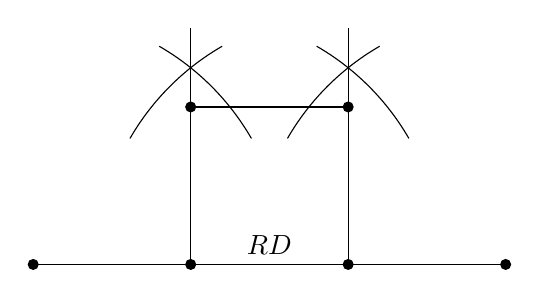
\begin{tikzpicture}
\draw (0,0) -- (6,0);
\foreach \i in {0,2,4,6}
  \fill (\i,0) circle (2pt);
\fill (2,2) circle (2pt);
\fill (4,2) circle (2pt);
\draw (2,2) -- (4,2);
\draw (2,0) -- (2,3);
\draw (4,0) -- (4,3);
\draw ([shift=(30:3.2cm)]0,0) arc (30:60:3.2cm);
\draw ([shift=(150:3.2cm)]4,0) arc (150:120:3.2cm);
\draw ([shift=(30:3.2cm)]2,0) arc (30:60:3.2cm);
\draw ([shift=(150:3.2cm)]6,0) arc (150:120:3.2cm);
\path (2,0) -- node[above] {$RD$} (4,0);
\end{tikzpicture}
\end{center}

\item \mbox{}
\[
\frac{355}{113}=3.14159292\,.
\]

\end{enumerate}

